\documentclass[a4paper]{IEEEtran}
\usepackage[T1]{fontenc}
\usepackage[utf8]{inputenc}
\usepackage[english]{babel}

\usepackage{authblk}
\usepackage{hyperref}
\usepackage{graphicx}
\usepackage{listings}
%\usepackage{amsmath}
\usepackage[cmex10]{amsmath}
\usepackage{amssymb}
%\usepackage{fullpage}
\usepackage{float}
\usepackage{url} \urlstyle{sf}

\usepackage{dashrule}

\usepackage{color}
\usepackage{subcaption}
\newcommand{\alert}[1]{\color{red}{#1}}
\newcommand{\greyout}[1]{\color{gray}{#1}}

\setlength{\parskip}{1em}

\title{Generating fluctuating workload for cloud elasticity simulation}
\author{
	\IEEEauthorblockN{Simon Bihel}
	\IEEEauthorblockA{(Student) Computer Science Department, ENS Rennes\\
	\href{mailto:simon.bihel@ens-rennes.fr}{simon.bihel@ens-rennes.fr}}
}


\begin{document}
\maketitle

\begin{abstract}
\end{abstract}

\begin{IEEEkeywords}
\end{IEEEkeywords}

\section{Introduction} \label{intro}
\cite{casanova:hal-01017319} \cite{Naskos2016} \cite{tighe2013towards} 
\cite{calheiros2011cloudsim}

\section{Background} \label{background}
	\begin{itemize}
		\item What's a cloud
		\item Minimizing the cost (in all forms) is a research challenge,
		particularly for fluctuating usage
		\item Different types of scaling
		\item Present the survey that has categorized these works
    \item How are they categorized
		\item Simulation isn't used that much and it would give a lot
		\item Say that it gives good overview of what is needed to simulate
		\item Say that it covered everything
	\end{itemize}
  
  Cloud computing is a model that makes available infrastructures, platforms
  and software with a pay-as-you-go subscription. It aims to reduce the cost
  with a layer of visualization that allows virtual resources to be
  dynamically adjusted and occupied on-demand. The problem of using the
  minimal resources for the current demand/usage is still a research
  challenge that spans all layers and applications. This dynamic management
  of clouds is called cloud elasticity.
  
  \cite{Naskos2016} has categorized works on cloud elasticity and allows to see
  which elements of a cloud infrastructure, platform or application/software are
  impacted. As it is for now most research works are evaluated on real clouds It
  is interesting for a distributed systems simulator to search what is needed
  for simulating cloud elasticity. If it is shown that research works on cloud
  elasticity can be evaluated on a simulator they would benefit from cost
  reduction, re-runable experiments, trust in results...
  
  In this survey proposals are categorized as follows. The scope is about what
  elements of a cloud the proposals work on. It can be the management of VMs,
  allocation of resources... Then there is the purpose of the proposal.
  Enhancing the \textit{performances} (to meet the SLA), reducing the
  \textit{energy consumption} footprint, being \textit{available} when needed
  and reducing the overall \textit{cost}. Another dimension is the decision
  making. This is what a proposal add to an existing cloud to pursue its
  purpose. In addition to the scope there is the elastic actions performed by
  the proposals. As the scope is about what elements of a cloud are concerned,
  the elastic action is about what is done to them. Then there is the provider
  dimension that tells if there is only one provider or multiple ones. At last
  there is the method used by the proposal to evaluate itself, through real
  cloud, simulation or emulation.
  
  The survey gives a good overview on what elements of a cloud are
  manipulated to achieve cloud elasticity.
  
  But in the end..
  // How can I be sure that it has covered all cases?
  
  As the proposals are on reacting to variating usage, simulators need a way
  to express this fluctuating workload. We worked on elastic tasks that model
  tasks that are triggered regularly and with a usage that fluctuates over
  time.

  
  \begin{figure*}
    \label{cloud_arch}
    \caption{http://cloud-simulation-frameworks.wikispaces.asu.edu/}
    \centering
    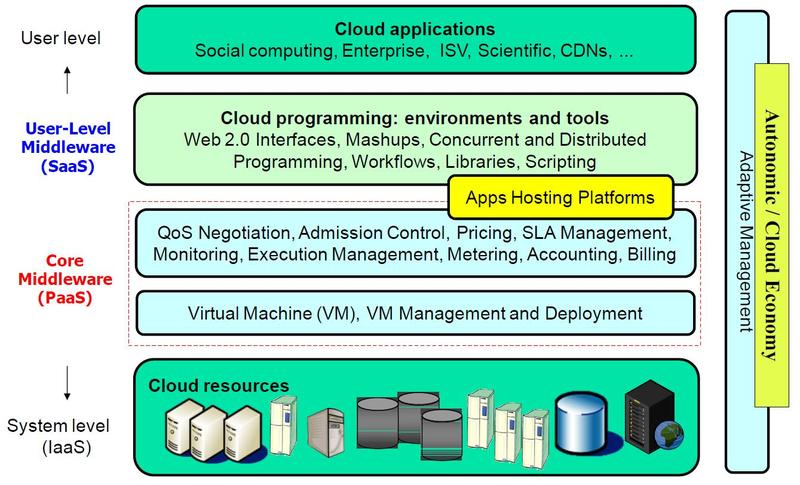
\includegraphics[width=0.8\textwidth]{../plots/cloud_architecture}
  \end{figure*}

\section{State of the art} \label{sota}
  \begin{itemize}
    \item Which elements have to be simulated and how do they work ?
    \item How workloads are generally modelized
    \item What others simulators have done
    \item What simulations for evaluation have been done
    \item What others evaluations do
  \end{itemize}
  
  Based on the classification of the survey, a simulator should allow the
  manipulation of scopes, the evaluation of the different purposes, make
  possible the elastic actions and allow multiple providers.
  
  // Tell that simgrid does all last 3 ?
  
  At the moment no simulator article talks about dynamic workload. On the other
  hand in the code of DCsim (\cite{tighe2013towards}) there was an interactive
  task and in the code of CloudSim (\cite{calheiros2011cloudsim}) there was an
  host with dynamic workload.
  
  // Go to contribution and go through each scope ?
  
  For en-actor scopes, the point of elastic tasks is just to generate usage
  so they can chose an application type depending on what kind of usage they
  want (cpu, disk...). For the different kinds of application type, elastic
  tasks have the same mechanism it is just the inherent micro-task that is
  repeated that changes. An elastic task will repeatedly execute an MSG task.
  Currently an MSG task can only simulate computing and message passing so
  only Multi-tier Applications can be simulated at the moment. Simulating
  disk and RAM usage would allow the simulation of databases, storage and
  thus generic application.
       

\section{Contribution} \label{contrib}
  What can my contribution do that is in the survey?
  \begin{itemize}
    \item Only computational tasks for now, might be able to do storage/DBs
    tasks in the future. Generic ones won't be possible unless you can pass a
    task directly to an ET.
    \item Need to use the host of a task when executing to allow vertical
    scaling and need to manage multiple hosts to allow horizontal scaling.
    \item Multiple provider is possible but has to be coded.
    \item Purpose?
  \end{itemize}

\section{Evaluation} \label{eval}
  \begin{itemize}
    \item How the experiments were made
  \end{itemize}
  \subsection{Raw performances}
    \begin{figure}
      \label{time_raw}
      \centering
      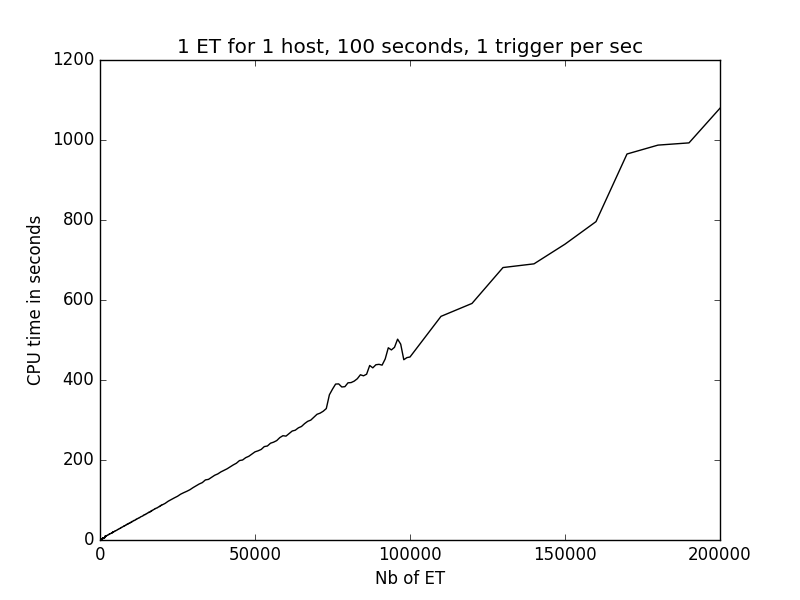
\includegraphics[width=0.55\textwidth]{../plots/raw_perf_time}
    \end{figure}
    \begin{figure}
      \label{mem_raw}
      \centering
      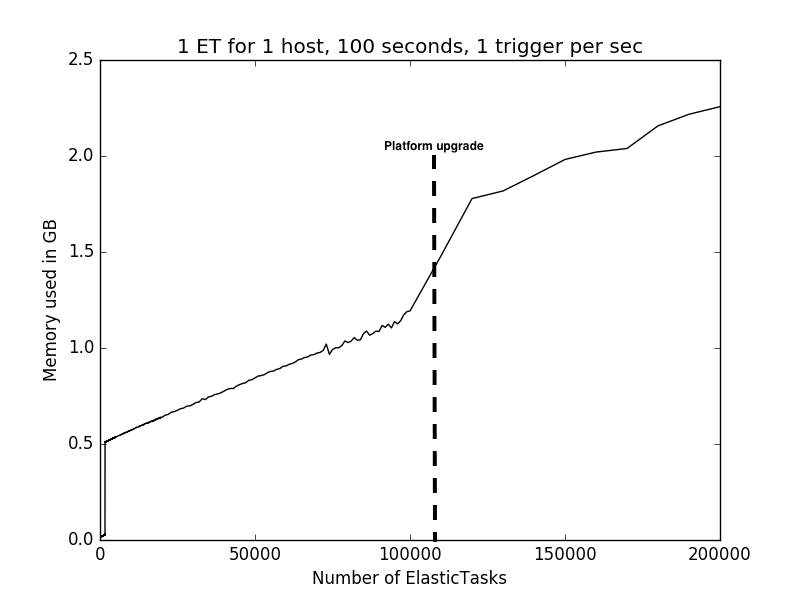
\includegraphics[width=0.55\textwidth]{../plots/raw_perf_mem}
    \end{figure}
  \subsection{Real traces}
  \subsection{Functionalities}

\section{Conclusion} \label{conclu}



\bibliographystyle{IEEEtran}
\bibliography{bibi}
\end{document}
